% 
% Annual Cognitive Science Conference
% Sample LaTeX Paper -- Proceedings Format
% 

\documentclass[10pt,letterpaper]{article}

\usepackage{cogsci}
\usepackage{pslatex}
\usepackage{apacite}
\usepackage{url}
\usepackage{graphicx}
\usepackage{caption}
\usepackage{subcaption}
\usepackage{listings}
\usepackage{color}
\usepackage{textcomp}
\usepackage{amsmath}
\usepackage{amssymb}
\usepackage{wrapfig}
\usepackage{lipsum}

\graphicspath{{figures/}}

\def\signed #1{{\leavevmode\unskip\nobreak\hfil\penalty50\hskip2em
  \hbox{}\nobreak\hfil(#1)%
  \parfillskip=0pt \finalhyphendemerits=0 \endgraf}}

\newsavebox\mybox
\newenvironment{aquote}[1]
  {\savebox\mybox{#1}\begin{quote}}
  {\signed{\usebox\mybox}\end{quote}}


\definecolor{Red}{RGB}{255,0,0}
\newcommand{\red}[1]{\textcolor{Red}{#1}}  


\title{It goes without saying: The pragmatics of backfiring utterances}

\author{{\large \bf Eleanor ChesTnut*} (eleanor.chestnut@stanford.edu) and {\large \bf Michael Henry Tessler*} (mtessler@stanford.edu) \\
  Department of Psychology, Stanford University}


\begin{document}

\maketitle


\begin{abstract}
Here is an abstract.

\textbf{Keywords:} 
pragmatics; language; common ground; Bayesian model

\end{abstract}

\section{Introduction}
In one of the most infamous moments in U.S. presidential history, Richard Nixon declared to the press corps, “I am not a crook” (CITE).  On the surface, this claim argues for Nixon’s innocence, as it literally states that he is not a crook.  As several researchers have shown, however, this statement contains a number of pragmatic implications that actually counter its literal, semantic meaning (CITE).  Nixon’s claim, for instance, presupposes that others believed that he was a crook; otherwise, it would not have been an informative statement to make, since most people presumably are not crooks (Grice, 1975).  Thus, if a listener is not aware of the Watergate scandal, or if they have no reason to question Nixon’s moral status, they might actually learn from this claim that Nixon was likely corrupt in some way.



\red{mht: streamline paragraphs 2 and 3 and make them into  the same paragraph}

To date, this inferential process, or “backfiring” linguistic effect, has received little attention in the literature.  In fact, most theories of language processing assert the opposite: if a person hears that Nixon is not a crook, then they should update their belief about Nixon to include this information... [EDIT].  A few studies, however, provide preliminary evidence that utterances that are redundant with a listener’s preexisting beliefs do cause listeners to search for ways to make those utterances informative \cite{Yandell1979, Wegner1981, Gruenfeld1992, Kravtchenko2015}.  This process ultimately undermines the utterances’ literal meanings.  
\citeA{Wegner1981}, for example, demonstrated that newspaper headlines such as “Bob Talbert is not linked to the Mafia” [CHECK] cause adults to have a more negative impression of Bob than they would otherwise, despite not explicitly asserting any incriminating information--indeed, despite denying incriminating information.  Here, since the default assumption is that people are not typically linked to the mafia, this headline is not immediately informative.  As a result, adults construct a context that would make the headline informative, namely, one in which Bob is known to be a bad person.  
\citeA{Gruenfeld1992} went even further to show that uninformative newspaper headlines can actually cause people to believe the exact opposite of what those headlines claim.  After reading the headline “Robert Kennedy was not planning the assassination of Fidel Castro”, for example, which denies a proposition that adults a priori should not believe, adults in their study more strongly believed that Robert Kennedy was planning to assassinate Fidel Castro.


\begin{figure}
\centering
    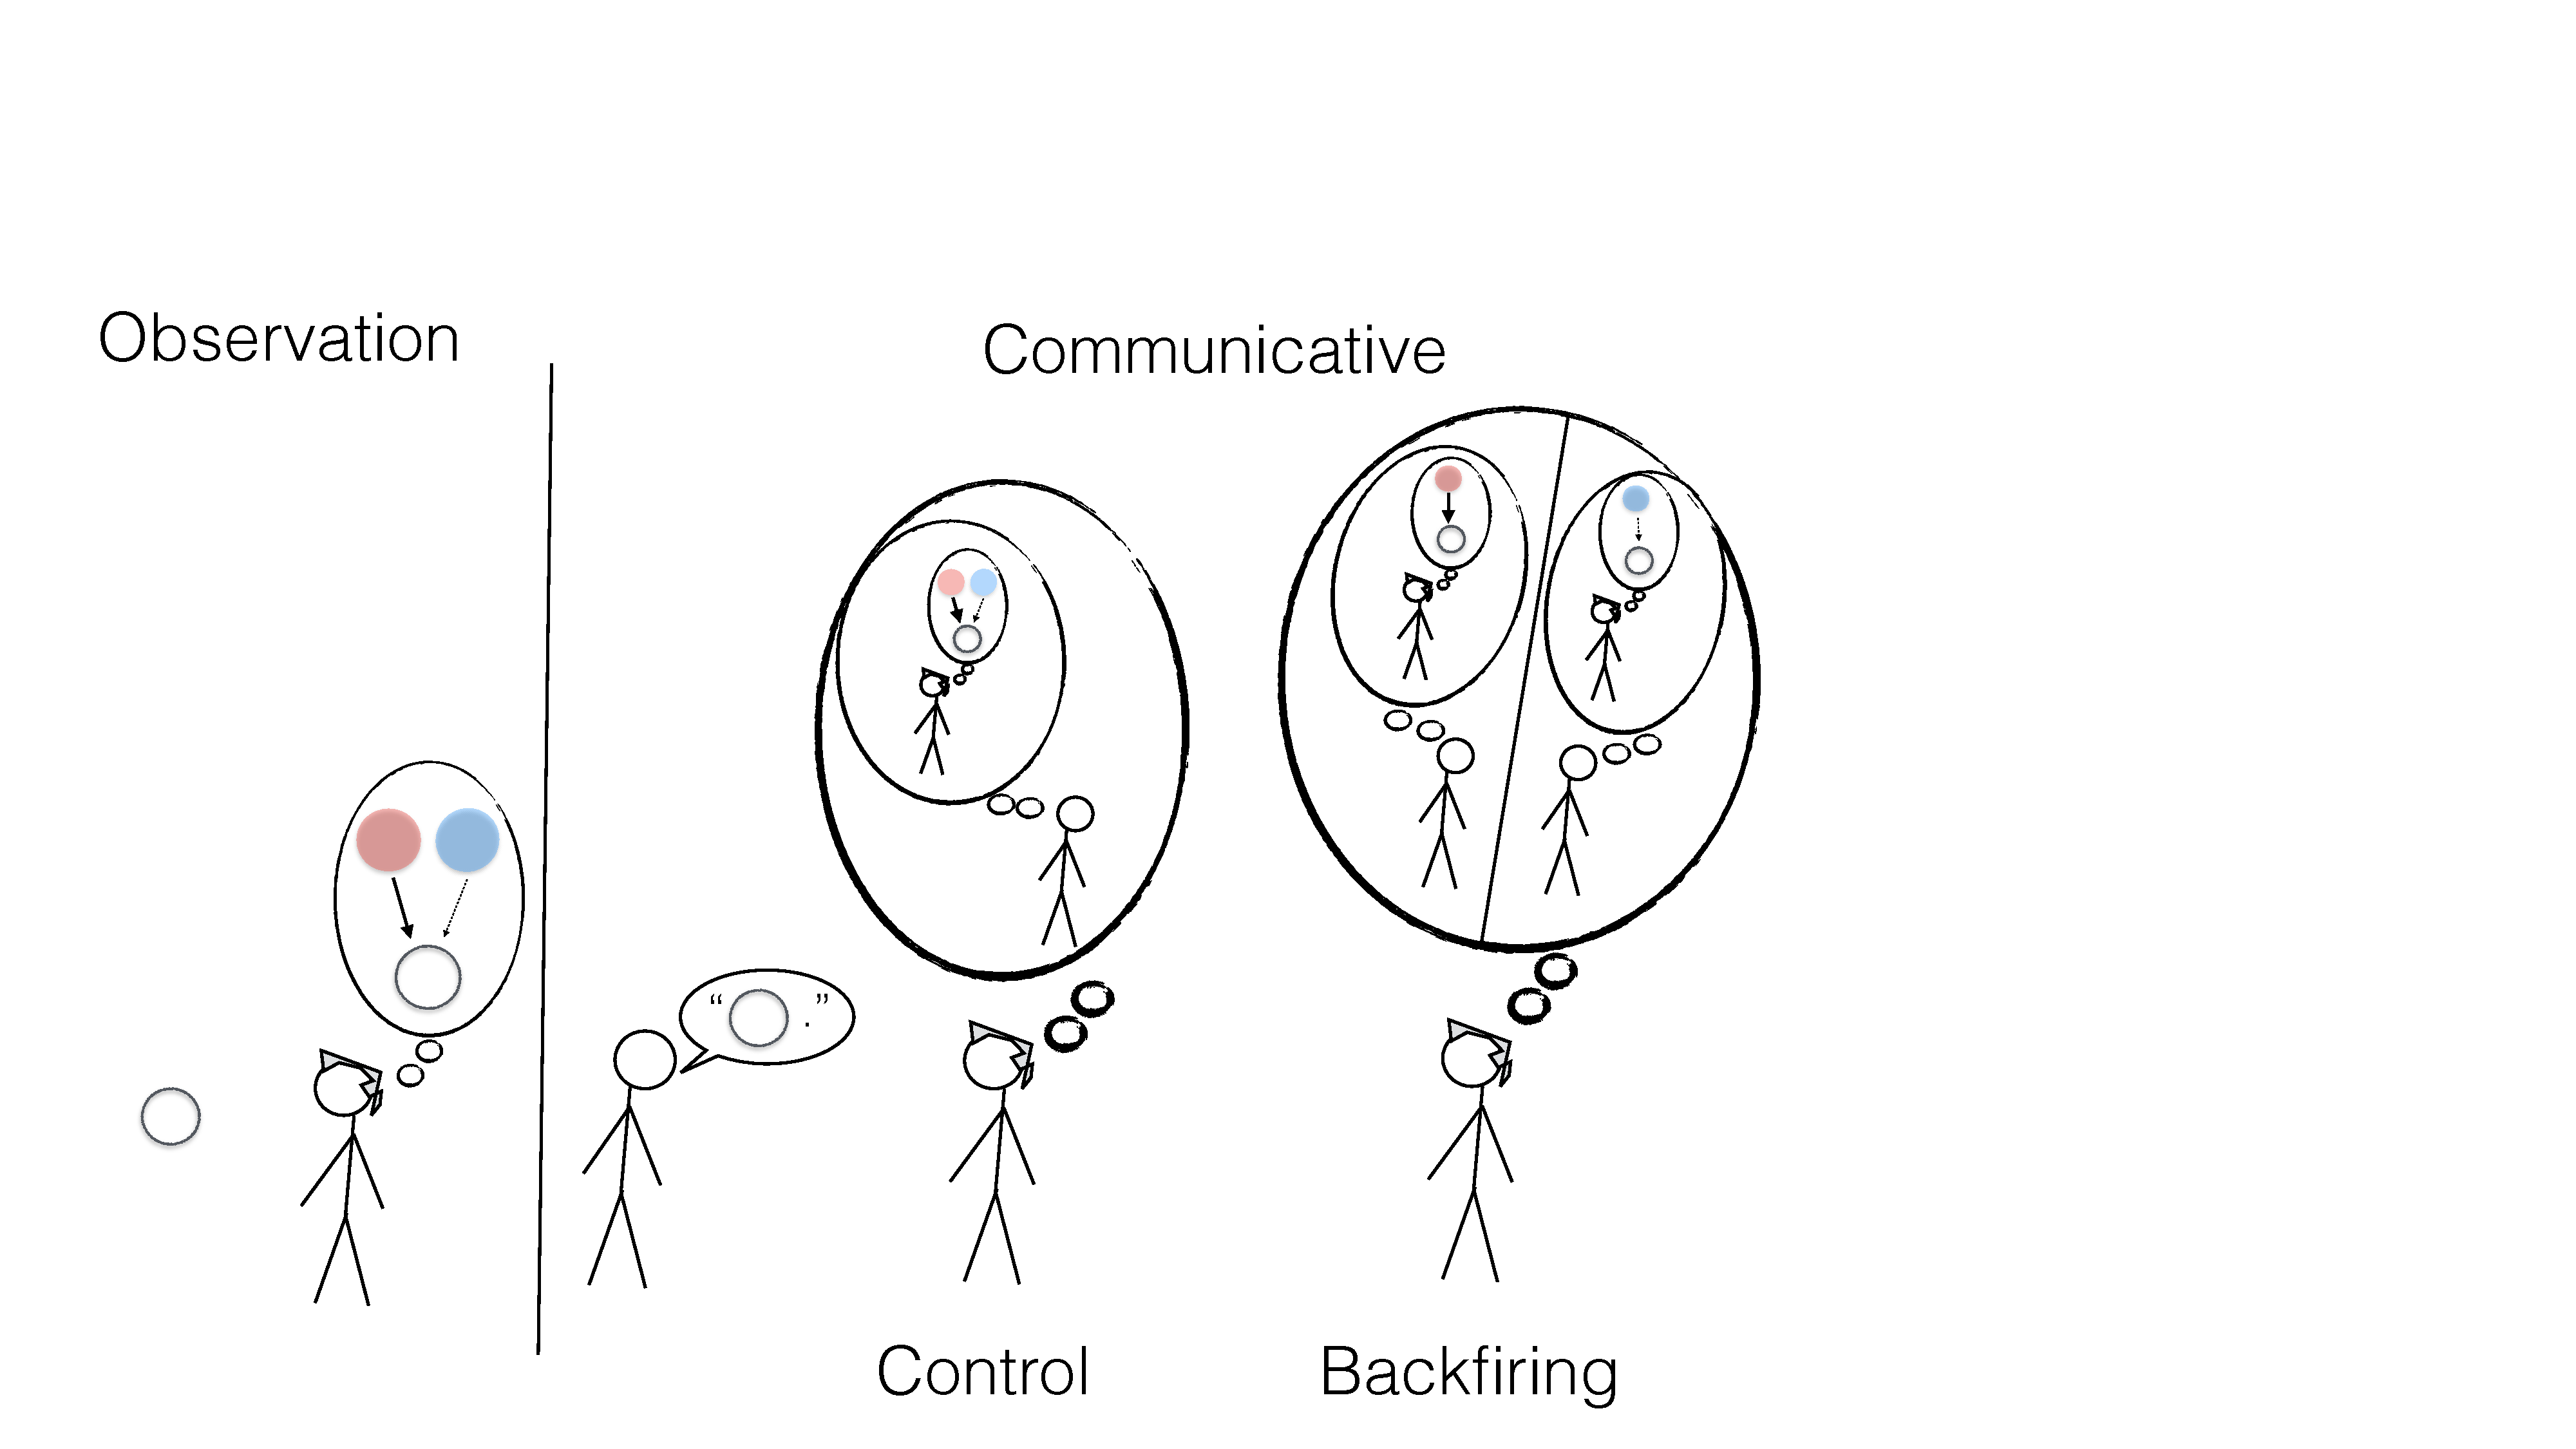
\includegraphics[width=\columnwidth]{cartoon}
    \caption{}
  \label{fig:cartoon}
\end{figure}


Affirming redundant information can have a similar effect \cite{Gruenfeld1992, Kravtchenko2015}.  
\citeA{Kravtchenko2015} for example, recently showed that if a speaker says, “John paid the cashier!” as part of a story about a trip to a grocery store, adults will infer that John does not typically pay cashiers.  This inference is based on the fact that paying cashiers is a standard part of buying groceries, and can easily be inferred without the speaker having to state it explicitly (Bower et al., etc.).  Thus, in an attempt to make the utterance informative, adults assume that paying cashiers must be uncharacteristic of John.  Critically, if the story begins by asserting that John is usually broke, then adults do not make this inference, because the idea of John paying the cashier is no longer redundant with their expectations.

To our knowledge, no current model of language processing can account for this pragmatic inference.  We propose such a model in the present study (brief description?).  In Experiment 1, we replicate previous findings that adults try to avoid redundancy in communicative contexts \cite{Kravtchenko2015} (also cite Jaeger studies etc.) and test whether our proposed model predicts these results.  [DEFINE COMMUNICATIVE CONTEXTS?] Specifically, we ask whether utterances such as, “My student turned in her homework on time today,” imply that the student does not typically turn in her homework on time, despite serving as evidence for this behavior.  We also test an important, previously unexplored(?) prediction of our model: that this “backfiring” effect of language should be eliminated when the utterance is no longer considered to be communicative.  Since this pragmatic inference depends on the conversational agreement that utterances should be maximally informative, when this conversational agreement is removed, adults should simply accept utterances at face value.



\section{A model of backfiring language}

Observing an event is often evidence for an underlying cause that could reliable give rise to the event.
For example, it is reasonable to fear a wet vacation when you disembark in your destination and find it raining.  [[THIS EXAMPLE IS CONFUSING TO ME]]
Similarly, observing a behavior can be taken as evidence for an underlying habit in a person. 
Seeing your friend's roommate doing her dishes provides some evidence that the roommate usually does her dishes. 
It is a more likely explanation than the alternative.

There is an interesting issue in communicative situations, however, because if an event always occurs, then----assuming the listener and speaker are in common ground about it---it is not informative to remark on it. 
A speaker who deliberately remarks ``My roommate did her dishes today.'' should believe that usually her roommate does not do her dishes, and believes his listener to believe this as well. 
A listener who does not actually know whether or not the speaker's roommate usually does her dishes will interpret the utterance as implicating that the roommate does not usually do her dishes.
We refer to the phenomena that a speech-act about an event can provide evidence against an underlying cause that would reliable give rise to the event as \emph{backfiring}. 

We formalize the backfiring inference as a probabilistic model of pragmatic communication where listener and speaker do not share common ground. 




\section{Experiment}

	In Experiment 1, we measured adults’ interpretations of affirmations (e.g., “My student turned in her homework on time today) in both communicative (e.g., two friends having a conversation) and non-communicative (e.g., two friends completing a survey together) contexts.  We predicted that in communicative contexts, adults should interpret the affirmations as expressing atypical behavior (e.g., the student does not typically turn in her homework on time), based on the tacit conversational agreement that utterances should be informative \cite{Grice1975}.  In non-communicative contexts, on the other hand, adults should interpret the utterance as reflecting typical behavior, since in these contexts there is no conversational pressure to be informative.  Instead, according to standard Bayesian reasoning(???), the affirmation should serve as evidence that the person does tend to engage in that behavior.

\subsection{Method}

\subsubsection{Participants}

Participants were XXXX.

\subsubsection{Materials}

A total of 64 trials were created, which consisted of four versions of sixteen items.  Each of these four versions corresponded to a different within-subjects condition: the Baseline condition, the Literal condition, the Speaker Manipulation(??) condition, and the Pragmatic condition.  Participants completed a series of 16 trials randomly drawn from this group of 64, which were evenly distributed across conditions and included only one version of each item (i.e., participants never saw two versions of the same item).  Trials were presented in random order.

Baseline condition. Trials in the Baseline condition were used to measure participants’ preexisting biases.  On one trial, for example, participants read the following scenario: “Molly is having a hard time remembering which student her officemate is tutoring.  She knows it is either Tom or Jim. Tom, she knows, always turns in his homework on time.  Jim, she knows, only occasionally turns in his homework on time.”  Participants then had to decide who they thought the officemate’s student was--Tom or Jim--without any other information and rate their confidence in their decision on a sliding scale.  All trials had the same structure: a character having trouble remembering information, and then a description of two options, one of which always engages in a behavior, and one of which only occasionally engages in a behavior.

Pragmatic condition. The Pragmatic condition was identical to the Baseline condition, except a brief utterance was added to the vignette after the description of the two options.  In the officemate scenario, for example, participants read, “In their office, Molly’s officemate says to her, ‘My student turned in his homework on time today.’”  We predicted that in this condition adults should be more likely to state, relative to baseline, that the officemate’s student is the one who only occasionally turns in his homework on time, since that context would make the utterance informative.

Literal condition. The Literal condition was the same as the Pragmatic condition, except an observation was added after the description of the two options rather than an utterance.  In the officemate scenario, this observation was, “In their office, Molly notices some papers on her officemate's desk. Her officemate's student turned in his homework on time today.”  Here, the same content is expressed--the student turned in his homework on time today--but it is no longer part of a conversation.  Thus, adults should be somewhat biased, relative to baseline, to select the student who always turns in his homework on time, since this evidence is most consistent with that behavior.

Speaker Manipulation condition.  The Speaker Manipulation condition was also the same as the Pragmatic condition, except the utterance added was no longer in a communicative context(??).  Participants read, for example, “In their office, Molly helps her officemate fill out a daily report card for her student, while her officemate files away some papers.  Molly reads out loud from the report card, ‘Did your student turn in his homework on time today?’  Her officemate replies, ‘Yes. My student turned in his homework on time today.’”  Because the sentence, “My student turned in his homework on time today,” is now a response to a question on a report card rather than a spontaneous communicative act, it does not have any pragmatic implications.  As a result, participants should again be somewhat biased to select the student who always turns in his homework on time.

\subsubsection{Procedure}

\subsection{Results}

(how to incorporate confidence ratings?)

The dependent measures were the proportion of times participants selected the option described as always engaging in the given behavior (need a better shorthand for this), and their confidence in that selection.  To determine how the Pragmatic, Literal, and Speaker Manipulation conditions compared to the Baseline condition, we fit the data using mixed-effects regression models comparing the responses and confidence ratings of the experimental conditions to those of the Baseline condition.  Each model had a fixed effect of condition and random effects of item and participant.  To test for the significance of effects, we performed likelihood ratio tests. Chi-squared values, degrees of freedom, and p-values, all from the likelihood ratio test, are reported for each statistical test.

As predicted, participants were significantly less likely to choose the “always” option in the Pragmatic condition (M = .46, SE = XX, n = XX) than in the Baseline condition (M = .71, SE = XX, n = XX) , χ2(1) = 81.15, p < .001.  Reading, for example, “My student turned in his homework on time today,” in a communicative context caused participants to infer that the student does not typically turn in his homework on time.  Adults were also more confident in their choices in the Pragmatic condition (M = .63, SE = XX, n = XX) than in the Baseline condition (M = .39, SE = XX, n = XX).

The Literal (M = .71, SE = XX, n = XX) and Speaker Manipulation (M = .68,  SE = XX, n = XX) conditions, however, did not differ significantly from the Baseline condition, χ2(1) = 0, p = .98, and χ2(1) = 2.11, p = .15, respectively, even though we expected participants in these conditions to be more likely to choose the “always” option.  One possibility is that for the items in this task, there was not much room for preference for the “always” option to strengthen, given that participants already preferred the “always” option in the Baseline condition at above-chance levels, t(119) = 9.05, p < .001.  Confidence ratings, however, did distinguish among these conditions.  Confidence ratings in both conditions (M = .60, SE = XX, n = XX in the Literal condition; M = .60, SE = XX, n = XX in the Speaker Manipulation condition) were significantly higher than confidence ratings in the Baseline condition,  χ2(1) = 275.41, p <.001, and χ2(1) = 255.68, p < .001, respectively.  Thus, the evidence provided in these two experimental conditions made adults at least more confident in their choices.  

POST-HOC ANALYSES?
To determine how pre-existing biases might influence participants’ responses in each of our conditions, we performed a median split analysis, separating items in the Baseline condition for which participants had weak preferences (M  = XXXX) from those for which participants had strong preferences (M = XXXX).  


\bibliographystyle{apacite}

\setlength{\bibleftmargin}{.125in}
\setlength{\bibindent}{-\bibleftmargin}

\bibliography{backfiring-cogsci2016}


\end{document}
